\documentclass[a4paper, 12pt]{extreport}
\usepackage[margin=1in]{geometry}
\usepackage{tikz}
\usepackage{setspace}
\graphicspath{ {../../resources/images/} }
\usepackage[titles]{tocloft}
\usepackage{titlesec}
\usepackage[hidelinks]{hyperref}
\usepackage{pdfpages}
\titleformat{\chapter}[hang]{\huge\bfseries}{\thechapter}{20pt}{\vspace{0.5em}}
\titlespacing*{\chapter}{0pt}{-3em}{1.1\parskip}
\usepackage[backend=biber, style=numeric, sorting=none]{biblatex}
\usepackage[nottoc,numbib]{tocbibind}
\renewbibmacro{finentry}{\finentry%
	\iffieldundef{annotation}
	{}
	{\par\medskip\printfield{annotation}\medskip\finentry}}

\addbibresource{../../resources/citation.bib}
\appto{\bibsetup}{\sloppy}

\begin{document}
	
	\onehalfspacing
	
	\begin{titlepage}
		
		\begin{tikzpicture}[remember picture, overlay]
			\node[xshift=14cm,yshift=-1.8cm,anchor=north west] at (current page.north west){%
			
\includegraphics[height=2.5cm]{logos/sunway}};
		\end{tikzpicture}
		
		\vfill
		
		\begin{center}
			\textbf{\large CAPSTONE PROJECT 1} \\
			\textbf{\large Activity Log} \\
			\vspace{1cm}
			\textbf{\large Evaluation of Nature-inspired Optimization\\Algorithms in Solving Versus Tetris}
			
			\vspace{1cm}
			
			by
			
			\vspace{1cm}
			
			\large Yap Wei Xiang \\
			21067939
			
			\vspace{1cm}
			
			\large Supervisor: Dr Richard Wong Teck Ken
			
			\vspace{1cm}
			
			\normalsize Semester: April 2024 \\
			Date: % DATE OF SUBMISSION
			
			\vfill
			
			Department of Computing and Information Systems\\
			School of Engineering and Technology\\
			Sunway University
		\end{center}
		
	\end{titlepage}
	
	\tableofcontents
	
	\chapter{Timeline}	
	\cite{tetris-is-hard-even-to-approx}

	\nocite{*}
	\printbibliography[heading={bibnumbered}, title={Bibliography}]
	
	\chapter{Meeting Records}
		
		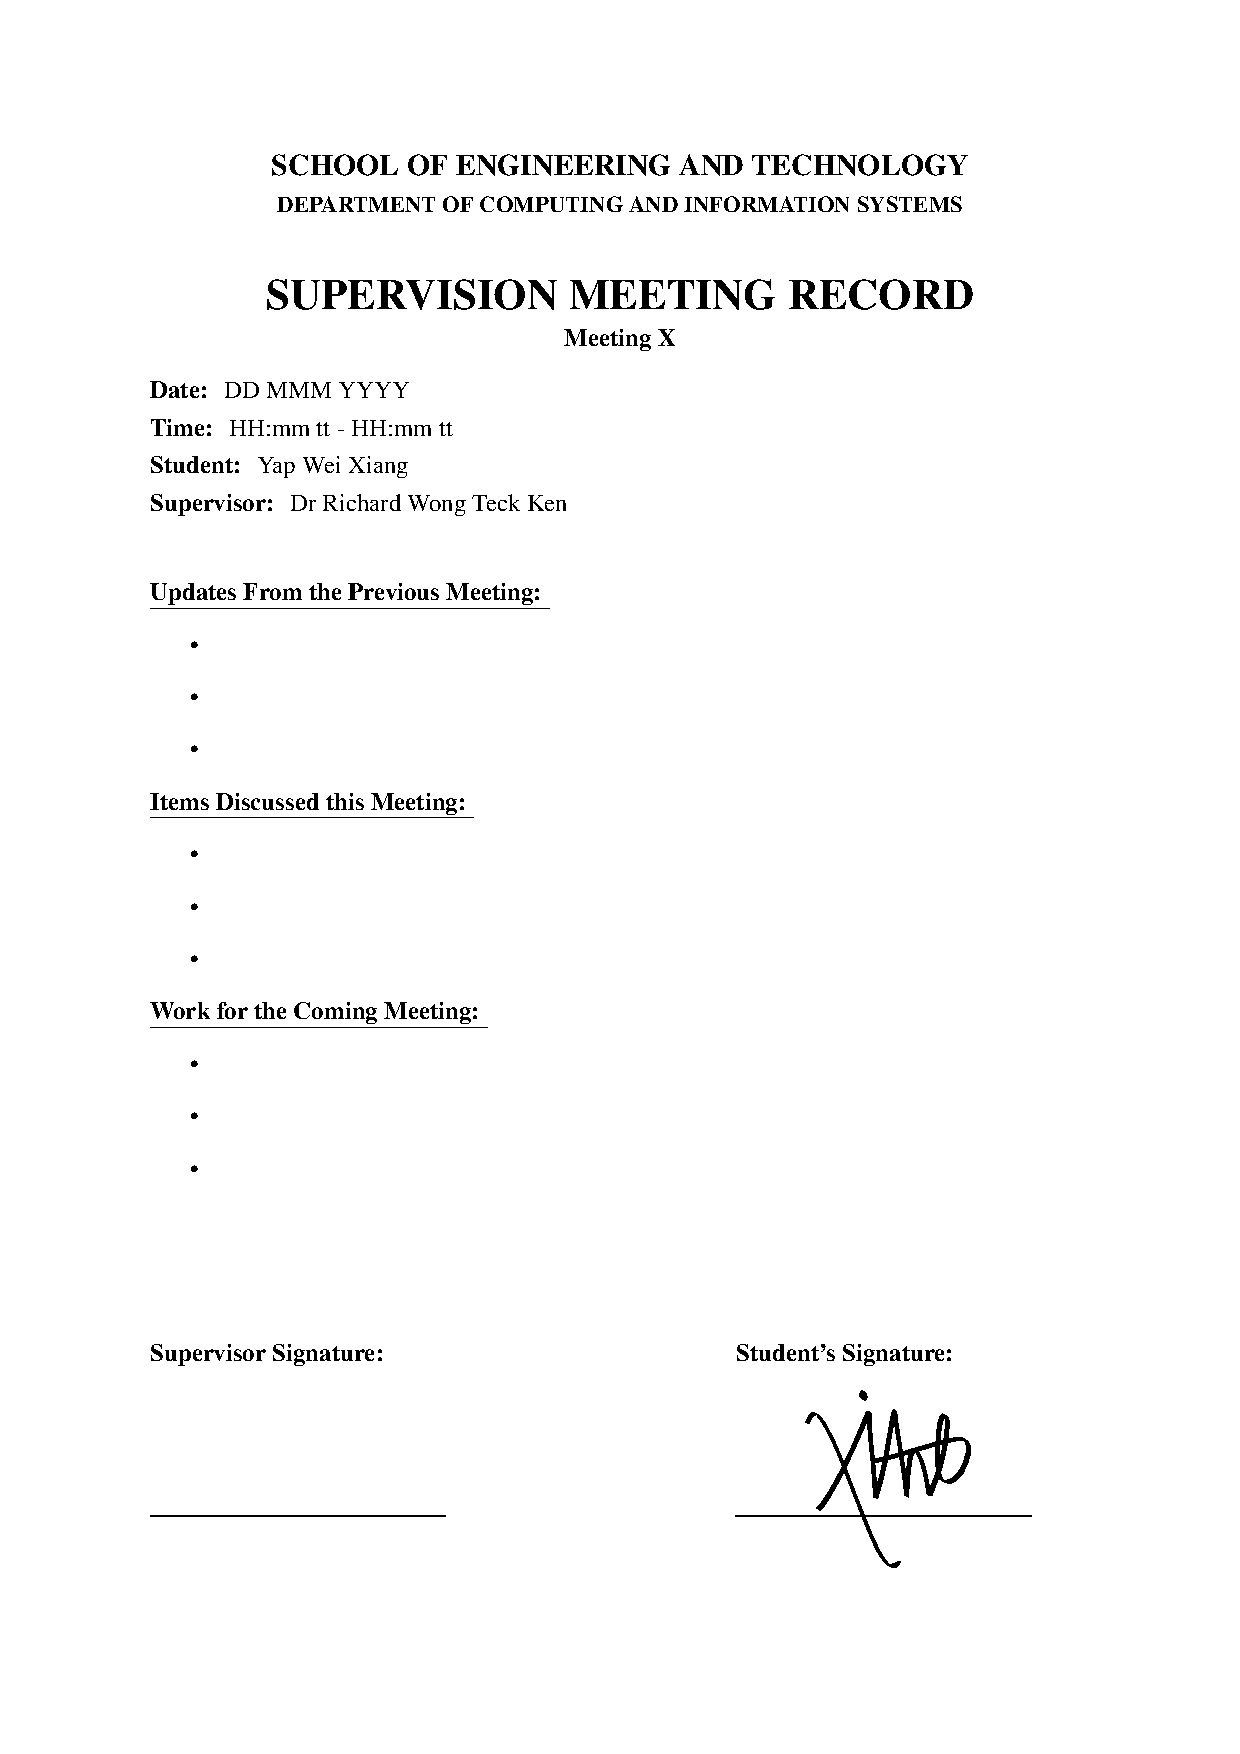
\includepdf[addtotoc={1, section, 1, Template, template1}, pagecommand={\thispagestyle{plain}}]{./meeting-records/template/meeting-record-template}
		
\end{document}